\hthree{Produktion}

Für die Produktion wird die Webseite für den Client einmal erstellt und als statische Dateien von NGINX bereitgestellt. Daher wird der Docker-Container für den Entwicklungs-Vite-Server nicht benötigt. Um die Daten der Datenbank zu persistieren, werden sie in einem Docker-Volume gespeichert. 

Allerdings werden für die Produktion Docker Images für die Rest API und den NGINX Webserver gebuildet. Dabei werden alle Dependencies installiert und der TypeScript-Code zu JavaScript transpiliert. Dadurch muss zum Starten nur mehr ein Container mit dem erstellten Image gestartet werden. Dabei ist es wichtig, dass Alle erforderlichen Environment Variablen gesetzt sind.

\begin{figure}[H]
    \centering
    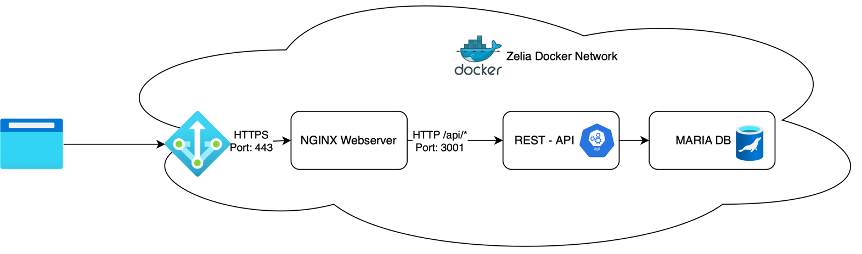
\includegraphics{media/Docker/ProdNetwork.png}
    \caption{Docker-Netzwerk für die Produktion}
\end{figure}

Da alle Container innerhalb des Zelia Docker Netzwerks liegen, ist es nicht möglich, dass direkt auf die Datenbank zugegriffen werden kann, da der einzig offene Port auf den NGINX Webserver verweist. 